\subsection{Problems}

\subsubsection{Design and describe an application-level protocol to be used between an automatic teller machine and a bank's centralized computer. Your protocol should allow a user's card and password to be verified, the account balance (which is maintained at the centralized computer) to be queried, and an account withdrawal to be made (that is, money disbursed to the user). Your protocol entities should be able to handle the all-too-common case in which there is not enough money in the account to cover the withdrawal. Specify your protocol by listing the messages exchanged and the action taken by the automatic teller machine or the bank's centralized computer on transmission and receipt of messages. Sketch the operation of your protocol for the case of a simple withdrawal with no errors, using a diagram similar to that in figures 1.2. Explicitly state the assumptions made by your protocol about the underlying end-to-end transport service. (P1)}

The protocol is implemented in the ATM and performs pattern-matching on the stated messages and performs the corresponding actions stated below (usually in the stated order).
\begin{enumerate}
    \item \texttt{HELLO <userid>}: Lets the ATM know that a card has been inserted and that the card belongs to the user with <userid>. The ATM them prompts for the corresponding password (PIN).
    \item \texttt{PWD <password>}: Lets the ATM know that the user has entered the password <password>. The ATM then sends <userid> and <password> to the bank's centralized computer and checks if there is a match. If not then it prompts for the password again for a for a maximum of 2 more times. If all 3 times are used then the ATM shuts down the connection and makes <userid> unable to establish a connection before they have been to the bank and reset their password.
    \item \texttt{BALANCE}: Requests the balance of the account belonging to <userid> from the bank's centralized computer. The ATM connects to the centralized computer and displays the balance for the user.
    \item \texttt{WITHDRAWAL <amount>}: Requests a withdrawal of <amount> from the account belonging to <userid> from the bank's centralized computer. The ATM connects to the centralized computer and checks if the account has enough money to cover the withdrawal. If not then the ATM displays an error message and prompts the user to enter a new amount. If the account has enough money then the ATM displays a message that the withdrawal was successful and prompts the user to take the money and the card.
    \item \texttt{BYE}: Lets the ATM know that the user has taken the card and the money and that the ATM can shut down the connection.
\end{enumerate}


\subsubsection{Equation 1.1 gives a formula for the end-to-end delay of sending one packet of length $L$ over $N$ links of transmission rate $R$. Generalize this formula for sending $P$ such packets back-to-back over the $N$ links. (P2)}
When there are $N$ links then there is $N-1$ routers between the source and destination of the $P$ packets. Assuming no delays and instantaneous propagation we have that at time $L/R$ the first packet have been sent from the source to the first router and is being transmitted to the same router, and at the same time the source is transmitting the second packet. At time 2L/R the first packet have been sent to the second router, the second packet has arrived at the first router and the source is transmitting the third packets. As described for equation 1.1. in KR, we have that this means that the first packet have arrived at the destination at $N \frac{L}{R}$. We also have that the $P$th packet is $P-1$ routers behind the first packet and that each router will take $L/R$ to traverse, meaning that the last packet arrives $(P-1) \frac{L}{R}$ after the first packet. Therefore the last packet will have arrived at time 
\begin{equation*}
    d_{\text{end-to-end}} = N \frac{L}{R} + (P-1) \frac{L}{R} = (N + P-1) \frac{L}{R}
\end{equation*}
which is by definition the end-to-end delay of sending $P$ packets back-to-back.


\subsubsection{Consider an aplication that transmits data at a steady rate (for example, the sender generates an $N$-bit unit of data every $k$ time units, where $k$ is small and fixed). Also, when such an application starts, it will continue running for a relatively long period of time. Answer the following questions, briefly justifying your answer: (P3)}

\textbf{a. Would a packet-switched network or a circuit-switched network be more appropriate for this application? Why?}\\
A circuit-switched network would be more appropriate, especially if it implemented with time-division multiplexing. This is because it allows the application to transmit over the bandwidth exactly when it needs to and only when it needs to. Since we know exactly when and how to the application needs to transmit we can allocate it to the application without any waste of bandwidth. Since the application is running for a relatively long period of time it reinforces this point since the overhead cost of setting up and tearing down connections are amortized over the lengthy period of a session. Packet-switched networks will provide more variable transmits, because it depends on the use of other users. Packet switching also have the risk of packet-loss etc. which might require packets to be retransmitted which ruins the strict transmitting policy of the application. \\
\\
\textbf{b. Suppose that a packet-switched network is used and the only traffic in this network comes from such applications as described above. Furthermore, assume that the sum of the application data rates is less than the capacities of each and every link. Is some form of congestion control needed? Why?}\\
No, if the sum of application data rates is less than the capacity of every link and since there is no bursts of transmission then we know that no packets will queue on any link. This causes no congestions and we do not need any congestion control under such conditions.



\subsubsection{Consider the circuit-switched network in Figure 1.13. Recall that there are four circuits on each link. Label the four switches A, B, C and D, going in the clockwise direction. (P4)}

\textbf{a. What is the maximum number of simultaneous connections that can be in progress at any one time in this network?}\\
Each switch have 4 links in each direction and if every switch pairs with any adjacent switch (say A-B, B-C, C-D, and D-A). Then each switch services all of its 4 links in each direction, yielding a total of 16 connections. \\
\\
\textbf{b. Suppose that all connections are between switches A and C. What is the maximum number of simultaneous connection that can be in progress?}\\
Since we only have 4 links, we use these 4 links to connect A and C, which results in a max of 4 simultaneous connections. \\
\\
\textbf{c. Suppose we want to make four connections between switches A and C, and another four connections between switches B and D. Can we route these calls through the four links to accommodate all eight connections?}\\
No. If we first make four connection between A and C, then we use all links that could otherwise go to B. If we instead first make four connections between B and D, then we use all links that could otherwise go to C. Therefore it is not possible to accommodate all eight connections. This is only possible when making connections that only use two switches as in the example given in answer of question a. 



\subsubsection{Review the car-caravan analogy in Section 1.4. Assume a propagation speed of 100 km/hour. (P5)}

The analogy assumes that the first car in a caravan to arrive at a tollbooth waits at the tollbooth for the remaining cars before servicing and passing through the tollbooth. The analogy also assumes that it takes a tollbooth 12 seconds to service a car. \\
\\
\textbf{a. Suppose the caravan travels 175 km, beginning in front of one tollbooth,
passing through a second tollbooth, and finishing just after a third tollbooth.
What is the end-to-end delay?} \\
The initial analogy assumes 10 cars. To service the cars and transmit them on the highway 3 times (transmission delay) it takes 
\begin{equation*}
    3 \cdot 10 \, \text{cars} \cdot 12 \, \text{s/cars} = 360 \, \text{s} = \frac{360 \, \text{s}}{60 \, \text{s/min}} =  6 \, min
\end{equation*}
Then to propagate them on the highway (propagation delay) it takes
\begin{equation*}
    \frac{175 \, \text{km}}{100 \, \text{km/h}} =  1.75 \, \text{h} = 1.75 \, \text{h} \cdot 60 \, \text{min/h} =  105 \, min
\end{equation*}
Here we have aggregated the two times the cars are propagated since this is equal to the sum of the two times they travel on the highway as we assume instant acceleration. Summing the delays we get that the total end-to-end-delay is $6 \, \text{min} + 105 \, \text{min} = 111 \, \text{min}$. \\
\\
\textbf{b. Repeat (a), now assuming that there are eight cars in the caravan instead
of ten.} \\
The time to propagate (propagation delay) the cars on the highway is the same as in (a) as every car accelerates instantly and at the same time. But the time to service the cars and transmit them on the highway 3 times (transmission delay) is now 
\begin{equation*}
    3 \cdot 8 \, \text{cars} \cdot 12 \, \text{s/cars} = 288 \, \text{s} = \frac{288 \, \text{s}}{60 \, \text{s/min}} =  4.8 \, min
\end{equation*}
Summing the propagation delay of 105 min and the new transmission delay of 4.8 min gives us a total end-to-end delay of $109.8 \, \text{min}$.

\subsubsection{This elementary problem begins to explore propagation delay and transmission delay, two central concepts in data networking. Consider two hosts, A and B, connected by a single link of rate $R$ bps. Suppose that the two hosts are separated by $m$ meters, and suppose the propagation speed along the link is $s$ meters/sec. Host A is to send a packet of size $L$ bits to Host B. (P6)}

\textbf{a. Express the propagation delay, $d_{\text{prop}}$, in terms of $m$ and $s$.} \\
\begin{equation*}
    d_{\text{prop}} = \frac{m}{s}
\end{equation*}
\\
\textbf{b. Determine the transmission time of the packet, $d_{\text{trans}}$, in terms of $L$ and $R$.} \\
\begin{equation*}
    d_{\text{trans}} = \frac{L}{R}
\end{equation*}
\\
\textbf{c. Ignoring processing and queuing delays, obtain an expression for the end-to-
end delay.} \\
\begin{equation*}
    d_{\text{end-to-end}} = d_{\text{trans}} + d_{\text{prop}} = \frac{L}{R} + \frac{m}{s}
\end{equation*}
\\
\textbf{d. Suppose Host A begins to transmit the packet at time $t = 0$. At time $t =
d_{\text{trans}}$, where is the last bit of the packet?} \\
The last bit has just left host A and is on the start of the link. \\
\\
\textbf{e. Suppose $d_{\text{prop}}$ is greater than $d_{\text{trans}}$. At time $t = d_{\text{trans}}$, where is the first
bit of the packet?} \\
If $d_{\text{prop}} > d_{\text{trans}}$ then it takes longer for the bits to propagate on the link than it takes for host A to transmission them on the link. In this case the first bit is still on the link at time $t = d_{\text{trans}}$. \\
\\
\textbf{f. Suppose $d_{\text{prop}}$ is less than $d_{\text{trans}}$. At time $t = d_{\text{trans}}$, where is the first
bit of the packet?} \\
In that takes it takes longer for host A to transmission the bits on the link than it takes for them to propagate on the link to host B. In that case the first bit will already have reached host B at time $t = d_{\text{trans}}$ \\
\\
\textbf{g. Suppose $s = 2.5 \cdot 10^8$, $L = 1500$ bytes, and $R = 10$ Mbps. Find the
distance $m$ so that $d_{\text{prop}}$ equals $d_{\text{trans}}$.} \\
We have that 
\begin{equation*}
\begin{split}
    d_{\text{prop}} &= d_{\text{trans}} \Longleftrightarrow \\
    \frac{m}{s} &= \frac{L}{R} \Longleftrightarrow \\
    m &= \frac{L}{R} \cdot s \Longleftrightarrow \\
    m &= \frac{1500 \cdot 8 \, \text{bits}}{10 \cdot 10^6\, \text{bits/sec}} \cdot 2.5 \cdot 10^8 \, \frac{\text{m}}{\text{sec}} = 300 \, 000 \, \text{m} = 300 \, \text{km}
\end{split}
\end{equation*}


\subsubsection{In this problem, we consider sending real-time voice from Host A to Host B over a packet-switched network (VoIP). Host A converts analog voice to a digital 64 kbps bit stream on the fly. Host A then groups the bits into 56-byte packets. There is one link between Hosts A and B; its transmission rate is 10 Mbps and its propagation delay is 10 msec. As soon as Host A gathers a packet, it sends it to Host B. As soon as Host B receives an entire packet, it converts the packet’s bits to an analog signal. How much time elapses from the time a bit is created (from the original analog signal at Host A) until the bit is decoded (as part of the analog signal at Host B)? (P7)}

First the bit is transformed to digital at host A taking $\frac{1}{64 \cdot 10^3}$ seconds. Then the bit is grouped into a packet of 56 bytes, meaning it has to wait for the remaining bits in this packet being converted to digital. The worst case of this waiting time is when the inspected bit is the first bit in the packet, which gives the worst runtime of $\frac{56 \cdot 8 - 1}{64 \cdot 10^3}$ seconds. Next the bit has to be transmitted with the packet taking $\frac{56 \cdot 8}{10 \cdot 10^6}$ seconds. Then the bit has to be propagated along with the packet taking $\frac{1}{10^3}$ seconds. We assume that the first bit to be packed by host A (as the inspected bit was in our worst-case scenario from before) is the first to be decoded into analog by host B. We also assume that host B decodes the digital signal as fast as host A encodes the analog signal to digital. This means that the time it takes host B to decode the bit is $\frac{1}{64 \cdot 10^3}$. Adding all these delays together we get 
\begin{equation*}
\begin{split}
    d &= \frac{56 \cdot 8}{64 \cdot 10^3} + \frac{56 \cdot 8}{10 \cdot 10^6} + \frac{10}{10^3} + \frac{1}{64 \cdot 10^3} \\
    &= 0.007 + 0.0000448 + 0.01 + 0.000015625 \\
    &= 0.0170604255 \, \text{s} \\
    &= 17.0604255 \, \text{ms}
\end{split}
\end{equation*}

\subsubsection{Suppose users share a 10 Mbps link. Also suppose each user requires 200 kbps when transmitting, but each user transmits only 10 percent of the time. (See the discussion of packet switching versus circuit switching in Section 1.3.) (P8)}

\textbf{a. When circuit switching is used, how many users can be supported?} \\
When circuit switching is used, bandwidth is allocated to the user whether the user transmits or not. We can therefore find the number of users that can be supported by dividing the total bandwidth by the amount required for a user.
\begin{equation*}
    \frac{10 \cdot 10^6 \, \text{bits/s}}{200 \cdot 10^3 \, \text{bits/s}} = 50
\end{equation*}
meaning that 50 users can be supported by circuit switching on this network.\\
\\
\textbf{b. For the remainder of this problem, suppose packet switching is used. Find the probability that a given user is transmitting.} \\
Since each user only transmits 10 percent of the time then the probability that a given user is transmitting must be 0.1. \\
\\
\textbf{c. Suppose there are 120 users. Find the probability that at any given time, exactly $n$ users are transmitting simultaneously. (Hint: Use the binomial distribution.)} \\
Using the binomial distribution with $p = 0.1$ (found in part b.) and $N = 120$ we get
\begin{equation*}
\begin{split}
    \P\lr{X = n} &= \binom{N}{n} p^n \lr{1 - p}^{N - n} \\
    &= \binom{120}{n} 0.1^n 0.9^{120 - n}
\end{split}
\end{equation*}
\\
\textbf{d. Find the probability that there are 51 or more users transmitting simultaneously.}
This is found by
\begin{equation*}
    \P \lr{X > 51} = 1 - \P \lr{X \leq 50}  = 1 - \sum_{n = 0}^{50} \P\lr{X = n}
\end{equation*}
since $X \in \Z^+$. Inserting the probability function found in part c we get
\begin{equation*}
\begin{split}
    \P \lr{X > 51} &= 1 - \sum_{n = 0}^{50} \binom{120}{n} 0.1^n 0.9^{120 - n} \\
    &= 3.22925 \cdot 10^{-6}
\end{split}
\end{equation*}

\subsubsection{Consider the discussion in Section 1.3 of packet switching versus circuit switching in which an example is provided with a 1 Mbps link. Users are generating data at a rate of 100 kbps when busy, but are busy generating data only with probability $p = 0.1$. Suppose that the 1 Mbps link is replaced by a 1 Gbps link. (P9)}

\textbf{a. What is $N$, the maximum number of users that can be supported simultaneously under circuit switching?} \\
This is found by 
\begin{equation*}
    \frac{1 \cdot 10^9}{100 \cdot 10^3} = 10000
\end{equation*}
\\
\textbf{b. Now consider packet switching and a user population of $M$ users. Give a formula (in terms of $p$, $M$, $N$) for the probability that more than $N$ users are sending data.} \\
We have that $X \in \Z^+$ so we can express the probability function as a binomial PDF
\begin{equation*}
\begin{split}
    \P \lr{X > N} &= \sum_{n = N + 1}^{M} \binom{M}{n} p^n (p - 1)^{M - n}
\end{split}
\end{equation*}

\subsubsection{Consider the network illustrated in Figure 1.16. Assume the two hosts on the left of the figure start transmitting packets of 1500 bytes at the same time towards Router B. Suppose the link rates between the hosts and Router A is 4-Mbps. One link has a 6-ms propagation delay and the other has a 2-ms propagation delay. Will queuing delay occur at Router A? (P10)}

From the 6-ms link we have an arrival rate of 6 ms for every packet making the traffic
\begin{equation*}
    \frac{1500 \cdot 8 \, \text{bits}}{6 \cdot 10^{-3} \, \text{s}} = 2 \text{Mb/s}
\end{equation*}
From the 2-ms link we can calculate the traffic by 
\begin{equation*}
    \frac{1500 \cdot 8 \, \text{bits}}{2 \cdot 10^{-3} \, \text{s}} = 6 \text{Mb/s}
\end{equation*}
The outgoing traffic from the link is equal to the link rate which is only 4 Mb/s. The incoming traffic is not larger than the outgoing when sent on the 6-ms delay link. However on the 2-ms delay link we have that the incoming traffic is larger than the outgoing, which means that queuing delay wil occur at router A.

\subsubsection{Consider the scenario in Problem P10 again, but now assume the links between the hosts and Router A have different rates $R_1$ and $R_2$ byte/s in addition
to different propagation delays $d_1$ and $d_2$. Assume the packet lengths for the two hosts are of $L$ bytes. For what values of the propagation delay will no queuing delay occur at Router A? (P11)}

Denote link 1 as the link with rate $R_1$ and propagation delay $d_1$ and link 2 as the link with rate $R_2$ and propagation delay $d_2$. We have that the incoming traffic for link 1 is $L/d_1$, so no queuing will occur as long as $L/d_1 < R_1$. Similarly we have that the incoming traffic for link 2 is $L/d_2$, so no queuing occurs when $L/d_2 < R_2$. We must have that both of these conditions hold, if no queuing delay is to occur at router A.


\subsubsection{Consider a client and a server connected through one router. Assume the router can start transmitting an incoming packet after receiving its first $h$ bytes instead of the whole packet. Suppose that the link rates are $R$ byte/s and that the client transmits one packet with a size of $L$ bytes to the server. What is the end-to-end delay? Assume the propagation, processing, and queuing delays are negligible. Generalize the previous result to a scenario where the client and the server are interconnected by N routers. (P12)}

We assume that $h < L$, from the words ''instead of the whole packet''. It takes $L/R$ seconds for the server to transmit the package, meaning that the router receives the packet after $L/R$ seconds. The router then transmits the first $h$ bytes of the packet which takes $h/R$ time, meaning that the client receives the first $h$ bytes after $L/R + h/R$ seconds. The router has to transmit the $h$ sized packets $L/h$ times, meaning that the total time it takes for the router to transmit the packet is $\frac{h}{R} \frac{L}{h} = \frac{L}{R}$. The end-to-end delay (i.e. time for the client to receive the whole packet) is therefore
\begin{equation*}
    d_{\text{end-to-end}} = 2 \frac{L}{R}
\end{equation*}
The router is in this scenario essentially splitting the packet up into $L/h$ sized packets. The last bit of the package is therefore arriving at the client at the same time as it would in the scenario of p.54 (router transmits whole packet) which describes equation 1.1. Therefore a client and a server connected by $N$ routers have the end-to-end delay
\begin{equation*}
    d_{\text{end-to-end}} = \lr{N + 1} \frac{L}{R}
\end{equation*}

\subsubsection{(a) Suppose N packets arrive simultaneously to a link at which no packets are currently being transmitted or queued. Each packet is of length L and the link has transmission rate R. What is the average queuing delay for the N packets? \\
(b) Now suppose that $N$ such packets arrive to the link every $LN/R$ seconds. What is the average queuing delay of a packet? (P13)}

\textbf{(a)}\\
The first packet will zero queuing time, since the queue is empty and the packet is ready to be sent right away. The second will have a queue time of $L/R$ equal to the time it takes for the first packet to be transmitted and the following third packet will have a queue time of $2L/R$ and so on. In general the $n$th packet will have a queuing delay of 
\begin{equation*}
    (n - 1) \frac{L}{R}
\end{equation*}
So the average queuing time for the N packets will be
\begin{equation*}
\begin{split}
    \overline{d}_{\text{queue}} &= \frac{1}{N} \sum_{n = 1}^N (n - 1) \frac{L}{R} \\
    &= \frac{L}{RN} \sum_{n = 1}^N (n - 1) \\
    &= \frac{L}{RN} \sum_{n = 1}^{N - 1} n \\
    &= \frac{L}{RN} \frac{N \lr{N - 1}}{2} \\
    &= \frac{L \lr{N - 1}}{2R}
\end{split}
\end{equation*}
where we have used that $\sum_{i = 1}^X i = \frac{X \lr{X + 1}}{2}$. \\
\\
\textbf{(b)}\\
It takes $LN/R$ to transmit all of the $N$ packets. This means that the buffer is empty whenever the next $N$ packets arrive. The average queuing delay over all batches of packets is therefore equal to the average queuing delay of one batch, which was found in part (a) to be $\frac{L \lr{N - 1}}{2R}$.


\subsubsection{Consider the queuing delay in a router buffer. Let $I$ denote traffic intensity; that is, $I=La/R$. Suppose that the queuing delay takes the form $IL/R (1-I)$ for $I<1$. (P14)}

\textbf{a. Provide a formula for the total delay, that is, the queuing delay plus the transmission delay.} \\
The transmission delay is defined by $L/R$ and the queuing delay is defined as $IL/R (1-I)$ for $I<1$. The total delay can therefore be expressed as
\begin{equation*}
\begin{split}
    d_{\text{end-to-end}} &= \frac{L}{R} + \frac{IL}{R \lr{1 - I}} \\
    &= \frac{L \lr{1 - I}}{R \lr{1 - I}} +  \frac{IL}{R \lr{1 - I}} \\
    &= \frac{L \lr{1 - I} + IL}{R \lr{1 - I}} \\
    &= \frac{L - LI + IL}{R \lr{1 - I}} \\
    &= \frac{L}{R \lr{1 - I}} \\
    &= \frac{L/R}{1 - I} \\
\end{split}
\end{equation*}
\\
\textbf{b. Plot the total delay as a function of $L/R$.} \\
\begin{center}
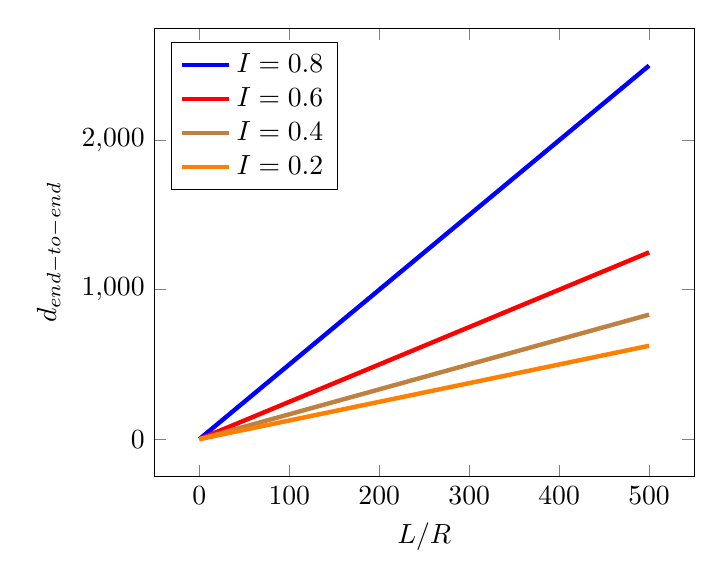
\begin{tikzpicture}
    \begin{axis}[domain=0:500, 
        samples=50, 
        legend pos=north west, 
        xlabel = $L/R$,
        ylabel = $d_{\text{end-to-end}}$]
        \addplot[blue, ultra thick] (x, x/0.2);
        \addlegendentry{$I = 0.8$}

        \addplot[red, ultra thick] (x, x/0.4);
        \addlegendentry{$I = 0.6$}

        \addplot[brown, ultra thick] (x, x/0.6);
        \addlegendentry{$I = 0.4$}

        \addplot[orange, ultra thick] (x, x/0.8);
        \addlegendentry{$I = 0.2$}
    \end{axis}
\end{tikzpicture}
\end{center}

\subsubsection{Let $a$ denote the rate of packets arriving at a link in packets/sec, and let $\mu$ denote the link's transmission rate in packets/sec. Based on the formula for the total delay (i.e., the queuing delay plus the transmission delay) derived in the previous problem, derive a formula for the total delay in terms of $a$ and $\mu$. (P15)}
Inserting $I = La/R$ and $\frac{R \, \text{bits/s}}{L \, \text{bits/packet}}= \mu \, \text{packet/s}$ into the formula for the total delay found P13 we get
\begin{equation*}
\begin{split}
    d_{\text{end-to-end}} &= \frac{L/R}{1 - I} \\
    &= \frac{L/R}{1 - La/R} \\
    &= \frac{1/\mu}{1 - a/\mu} \\
    &= \frac{1}{\mu - a}
\end{split}
\end{equation*}
which express the delay in terms of $a$ and $\mu$.

\subsubsection{Consider a router buffer preceding an outbound link. In this problem, you will use Little's formula, a famous formula from queuing theory. Let $N$ denote the average number of packets in the buffer plus the packet being transmitted. Let $a$ denote the rate of packets arriving at the link. Let $d$ denote the average total delay (i.e., the queuing delay plus the transmission delay) experienced by a packet. Little's formula is $N=a \cdot d$. Suppose that on  average, the buffer contains 100 packets, and the average packet queuing delay is 20 msec. The link's transmission rate is 100 packets/sec. Using  Little's formula, what is the average packet arrival rate, assuming there is  no packet loss? (P16)}

Isolating $a$ in Little's formula gives us
\begin{equation*}
    a = \frac{N}{d} 
\end{equation*}
we have that $N = 100$ packets/sec and $d = 0.02 \, \text{s}+ \frac{100 \, \text{packets}}{100 \, \text{packets/sec}} = 1.02$ sec. Inserting these values gives
\begin{equation*}
    a = \frac{100}{1.02} = 98.039
\end{equation*}
so the average packet arrival rate is 98.039 packets/sec.

\subsubsection{Consider the network illustrated in Figure 1.12. Would Equation 1.2 hold in such a scenario? If so, under which conditions? If not, why? (Assume $N$ is the number of links between a source and a destination in the figure.) (P17)}

The network in figure 1.12 illustrates how packets can queue up in a router when they arrive faster than they are transmitted (congestion). Equation 1.2 is $d_{\text{end-to-end}} = N \lr{d_{\text{proc}} + d_{\text{trans}} + d_{\text{prop}}}$ meaning that equation 1.2 assumes no congestion and therefore that queue delay is negligible. Equation 1.2 therefore only holds for the network in figure 1.1.2 under the condition that no congestion occurs in the network.


\subsubsection{Perform a Traceroute between source and destination on the same continent at three different hours of the day. (P18)}
First traceroute to UK at 18:30:
\begin{verbatim}
    % traceroute -I gov.uk         
    traceroute: Warning: gov.uk has multiple addresses; using 151.101.192.144
    traceroute to gov.uk (151.101.192.144), 64 hops max, 72 byte packets
     1  192.168.0.1 (192.168.0.1)  3.716 ms  2.068 ms  1.953 ms
     2  10.5.13.1 (10.5.13.1)  2.592 ms  9.268 ms  2.771 ms
     3  10.0.0.3 (10.0.0.3)  2.207 ms  2.143 ms  2.118 ms
     4  rasmusnielsenkollegiet.kbh-kua.core.fsknet.dk (130.226.217.193)  26.192 ms  
     29.797 ms  3.228 ms
     5  kbh-kua.ore.core.fsknet.dk (130.226.217.165)  2.386 ms  2.580 ms  2.723 ms
     6  dk-ore.nordu.net (109.105.102.160)  3.135 ms  2.888 ms  4.222 ms
     7  se-sthb.nordu.net (109.105.97.131)  19.990 ms  12.638 ms  13.773 ms
     8  se-bma.nordu.net (109.105.101.63)  11.224 ms  15.077 ms  11.652 ms
     9  as54113-1-100g-sk1.sthix.net (192.121.80.71)  19.065 ms  17.677 ms  19.923 ms
    10  151.101.192.144 (151.101.192.144)  19.691 ms  11.025 ms  14.791 ms
\end{verbatim}
Second traceroute to UK at 14:00:
\begin{verbatim}
    % traceroute -I gov.uk
    traceroute: Warning: gov.uk has multiple addresses; using 151.101.64.144
    traceroute to gov.uk (151.101.64.144), 64 hops max, 72 byte packets
     1  10.8.0.1 (10.8.0.1)  3.925 ms  4.567 ms  2.614 ms
     2  10.0.0.3 (10.0.0.3)  1.936 ms  2.256 ms  1.879 ms
     3  rasmusnielsenkollegiet.kbh-kua.core.fsknet.dk (130.226.217.193)  4.885 ms  
     4.215 ms  6.462 ms
     4  kbh-kua.ore.core.fsknet.dk (130.226.217.165)  3.364 ms  3.250 ms  3.097 ms
     5  dk-ore.nordu.net (109.105.102.160)  3.396 ms  3.690 ms  3.435 ms
     6  se-sthb.nordu.net (109.105.97.131)  11.425 ms  11.744 ms  11.497 ms
     7  se-kst.nordu.net (109.105.101.5)  12.650 ms  12.069 ms  11.620 ms
     8  as54113-2-100g-sk1.sthix.net (192.121.80.72)  25.837 ms  25.674 ms  25.887 ms
     9  151.101.64.144 (151.101.64.144)  11.489 ms  11.772 ms  11.753 ms
\end{verbatim}
Third traceroute to UK at 16:20:
\begin{verbatim}
    % traceroute -I gov.uk     
    traceroute: Warning: gov.uk has multiple addresses; using 151.101.0.144
    traceroute to gov.uk (151.101.0.144), 64 hops max, 72 byte packets
     1  10.8.0.1 (10.8.0.1)  9.911 ms  3.054 ms  8.821 ms
     2  10.0.0.3 (10.0.0.3)  2.316 ms  2.798 ms  2.629 ms
     3  rasmusnielsenkollegiet.kbh-kua.core.fsknet.dk (130.226.217.193)  32.219 ms  
     51.773 ms  27.735 ms
     4  kbh-kua.ore.core.fsknet.dk (130.226.217.165)  3.543 ms  6.770 ms  4.309 ms
     5  dk-ore.nordu.net (109.105.102.160)  3.133 ms  2.619 ms  3.005 ms
     6  se-sthb.nordu.net (109.105.97.131)  10.532 ms  11.647 ms  11.458 ms
     7  se-kst.nordu.net (109.105.101.1)  11.309 ms  11.988 ms  11.355 ms
     8  as54113-2-100g-sk1.sthix.net (192.121.80.72)  12.061 ms  12.802 ms  12.829 ms
     9  151.101.0.144 (151.101.0.144)  13.070 ms  12.002 ms  11.445 ms
\end{verbatim}
\textbf{a. Find the average and standard deviation of the round-trip delays at each of the three hours.} \\
Denote the vector of RTTs (round trip times) of the first traceroute as 
\begin{equation*}
\begin{split}
    \mathbf{X}_1 = &[
        3.716, 2.068, 1.953,
        2.592, 9.268, 2.771,
        2.207, 2.143, 2.118,
        26.192, 29.797, 3.228,
        2.386, 2.580, 2.723, \\
        &3.135, 2.888, 4.222,
        19.990, 12.638, 13.773,
        11.224, 15.077, 11.652,
        19.065, 17.677, 19.923,
        19.691, \\
        &11.025, 14.791
    ]
\end{split}
\end{equation*}
Then the average is $\overline{\mathbf{X}}_1 = 9.75$ and the standard deviation is $\sigma_{\mathbf{X}_1} = 8.09$. \\
\\
Denote the vector of RTTs of the second traceroute as
\begin{equation*}
\begin{split}
    \mathbf{X}_2 = &[
        3.925, 4.567, 2.614,
        1.936, 2.256, 1.879,
        4.885, 4.215, 6.462,
        3.364, 3.250, 3.097, \\
        &3.396, 3.690, 3.435,
        11.425, 11.744, 11.497,
        12.650, 12.069, 11.620,
        25.837, 25.674, 25.887,
        11.489, \\
        &11.772, 11.753
    ]
\end{split}
\end{equation*}
Then the average is $\overline{\mathbf{X}}_2 = 8.76$ and the standard deviation is $\sigma_{\mathbf{X}_2} = 7.16$. \\
\\
Denote the vector of RTTs of the third traceroute as
\begin{equation*}
\begin{split}
    \mathbf{X}_3 = &[
        9.911, 3.054, 8.821,
        2.316, 2.798, 2.629,
        32.219, 51.773, 27.735,
        3.543, 6.770, 4.309, \\
        &3.133, 2.619, 3.005,
        10.532, 11.647, 11.458,
        11.309, 11.988, 11.355,
        12.061, 12.802, 12.829,
        13.070, \\
        &12.002, 11.445
    ]
\end{split}
\end{equation*}
Then the average is $\overline{\mathbf{X}}_3 = 11.38$ and the standard deviation is $\sigma_{\mathbf{X}_3} = 10.54$. \\
\\
\textbf{b. Find the number of routers in the path at each of the three hours. Did the paths change during any of the hours?} \\
The first traceroute passes through 9 routers while the second and third passed through 9 routers. The paths must therefore have changed, which is probably because the first traceroute was performed on a different day than the day I performed the second and third traceroutes. \\
\\
\textbf{c. Try to identify the number of ISP networks that the Traceroute packets pass through from source to destination. Routers with similar names and/or similar IP addresses should be considered as part of the same ISP. In your experiments, do the largest delays occur at the peering interfaces between adjacent ISPs?} \\
Names including nordu seems to be from the same ISP. It does seem that the largest delays happen when switching between different ISP-routers. \\
\\
\textbf{d. Repeat the above for a source and destination on different continents. Compare the intra-continent and inter-continent results.} \\
First traceroute from Denmark to Japan at 18:30:
\begin{verbatim}
    % traceroute -I japan.go.jp
    traceroute: Warning: japan.go.jp has multiple addresses; using 18.173.5.29
    traceroute to japan.go.jp (18.173.5.29), 64 hops max, 72 byte packets
     1  192.168.0.1 (192.168.0.1)  3.595 ms  2.183 ms  2.009 ms
     2  10.5.13.1 (10.5.13.1)  2.750 ms  2.342 ms  2.356 ms
     3  10.0.0.3 (10.0.0.3)  2.039 ms  6.423 ms  2.322 ms
     4  rasmusnielsenkollegiet.kbh-kua.core.fsknet.dk (130.226.217.193)  4.332 ms  
     8.136 ms  7.743 ms
     5  kbh-kua.ore.core.fsknet.dk (130.226.217.165)  2.829 ms  2.856 ms  2.822 ms
     6  dk-ore.nordu.net (109.105.102.160)  3.135 ms  3.399 ms  3.399 ms
     7  dk-bal2.nordu.net (109.105.97.249)  3.499 ms  3.240 ms  3.624 ms
     8  dk-bal.nordu.net (109.105.97.48)  3.463 ms  3.461 ms  3.367 ms
     9  ndn-gw.amazon.com (109.105.98.227)  3.854 ms  3.318 ms  3.668 ms
\end{verbatim}
Second traceroute to Japan at 14:00:
\begin{verbatim}
    % traceroute -I japan.go.jp
    traceroute: Warning: japan.go.jp has multiple addresses; using 18.173.5.17
    traceroute to japan.go.jp (18.173.5.17), 64 hops max, 72 byte packets
     1  10.8.0.1 (10.8.0.1)  3.747 ms  2.488 ms  2.960 ms
     2  10.0.0.3 (10.0.0.3)  2.019 ms  2.002 ms  2.425 ms
     3  rasmusnielsenkollegiet.kbh-kua.core.fsknet.dk (130.226.217.193)  5.021 ms  
     8.438 ms  7.743 ms
     4  kbh-kua.ore.core.fsknet.dk (130.226.217.165)  2.675 ms  4.018 ms  2.508 ms
     5  dk-ore.nordu.net (109.105.102.160)  2.445 ms  2.520 ms  2.936 ms
     6  dk-bal2.nordu.net (109.105.97.249)  3.061 ms  2.909 ms  3.384 ms
     7  dk-bal.nordu.net (109.105.97.48)  3.169 ms  2.850 ms  3.438 ms
     8  ndn-gw.amazon.com (109.105.98.227)  10.382 ms  3.016 ms  3.706 ms
     9  * * *
    10  * * *
    11  * * *
    12  * * *
    13  * * *
    14  52.93.139.249 (52.93.139.249)  4.100 ms  3.657 ms  4.080 ms
    15  server-18-173-5-17.cph50.r.cloudfront.net (18.173.5.17)  3.479 ms  3.629 ms  
    3.384 ms
\end{verbatim}
Third traceroute to Japan at 16:20:
\begin{verbatim}
    % traceroute -I japan.go.jp
    traceroute: Warning: japan.go.jp has multiple addresses; using 18.173.5.104
    traceroute to japan.go.jp (18.173.5.104), 64 hops max, 72 byte packets
     1  10.8.0.1 (10.8.0.1)  4.317 ms  3.078 ms  4.614 ms
     2  10.0.0.3 (10.0.0.3)  2.441 ms  2.838 ms  2.317 ms
     3  rasmusnielsenkollegiet.kbh-kua.core.fsknet.dk (130.226.217.193)  44.191 ms  
     25.895 ms  8.237 ms
     4  kbh-kua.ore.core.fsknet.dk (130.226.217.165)  3.591 ms  3.143 ms  3.096 ms
     5  dk-ore.nordu.net (109.105.102.160)  3.236 ms  3.269 ms  2.965 ms
     6  dk-bal2.nordu.net (109.105.97.249)  3.427 ms  3.685 ms  40.914 ms
     7  dk-bal.nordu.net (109.105.97.48)  3.428 ms  3.624 ms  3.357 ms
     8  ndn-gw.amazon.com (109.105.98.227)  3.666 ms  3.820 ms  3.416 ms
     9  * * *
    10  * * *
    11  * * *
    12  * * *
    13  * * *
    14  52.93.139.249 (52.93.139.249)  6.761 ms  3.785 ms  3.631 ms
    15  server-18-173-5-104.cph50.r.cloudfront.net (18.173.5.104)  4.741 ms  3.155 ms  
    2.952 ms
\end{verbatim}
Denote the vector of RTTs of the first japanese traceroute by
\begin{equation*}
\begin{split}
    \mathbf{Z}_1 = &[
        3.595, 2.183, 2.009,
        2.750, 2.342, 2.356,
        2.039, 6.423, 2.322,
        4.332, 8.136, 7.743,
        2.829, 2.856, 2.822, \\
        &3.135, 3.399, 3.399,
        3.499, 3.240, 3.624,
        3.463, 3.461, 3.367,
        3.854, 3.318, 3.668
    ]
\end{split}
\end{equation*}
Then the average RTT of the first traceroute is $\overline{Z}_1 = 3.56$ and the standard deviation is $\sigma_{Z_1} = 1.50$. \\
\\
Denote the vector of RTTs of the second japanese traceroute by
\begin{equation*}
\begin{split}
    \mathbf{Z}_2 = &[
        3.747, 2.488, 2.960,
        2.019, 2.002, 2.425,
        5.021, 8.438, 7.743,
        2.675, 4.018, 2.508,
        2.445, 2.520, 2.936, \\
        &3.061, 2.909, 3.384,
        3.169, 2.850, 3.438,
        10.382, 3.016, 3.706,
        4.100, 3.657, 4.080,
        3.479, 3.629, 3.384
    ]
\end{split}
\end{equation*}
Then the average RTT of the second traceroute is $\overline{Z}_2 = 3.74$ and the standard deviation is $\sigma_{Z_2} = 1.86$. \\
\\
Denote the vector of RTTs of the third japanese traceroute by
\begin{equation*}
\begin{split}
    \mathbf{Z}_3 = &[
        4.317, 3.078, 4.614,
        2.441, 2.838, 2.317,
        44.191, 25.895, 8.237,
        3.591, 3.143, 3.096,
        3.236, 3.269, 2.965, \\
        &3.427, 3.685, 40.914,
        3.428, 3.624, 3.357,
        3.666, 3.820, 3.416,
        6.761, 3.785, 3.631,
        4.741, 3.155, 2.952
    ]
\end{split}
\end{equation*}
Then the average RTT of the third traceroute is $\overline{Z}_3 = 7.05$ and the standard deviation is $\sigma_{Z_3} = 10.36$. \\
\\
The path of first japanese traceroute consists of 9 routers while (not counting the timeouts) the second the third traceroute had a path if 10 paths. The difference in routers might be explained by the fact that the second on third traceroute was performed on one day and the first traceroute on another. \\
\\
On the traceroutes to japan we see that amazon is used as an ISP to go to Japan. It is also the transition from this ISP to the next that causes the biggest delays (and a couple of timeouts).

\subsubsection{Metcalfe's law states the value of a computer network is proportional to the square of the number of connected users of the system. Let $n$ denote the number of users in a computer network. Assuming each user sends one message to each of the other users, how many messages will be sent? Does your answer support Metcalfe's law? (P19)}

If $n$ users each send a message to every other $n - 1$ users then the messages sent wil be $n(n- 1) = n^2 - n$. This means that the number of messages sent is proportional to $n$ the users in the network, which supports Metcalfe's law, if the value of a computer network is proportional to the messages sent.


\subsubsection{Consider the throughput example corresponding to Figure 1.20(b). Now suppose that there are $M$ client-server pairs rather than 10. Denote $R_s$, $R_c$, and $R$ for the rates of the server links, client links, and network link. Assume all other links have abundant capacity and that there is no other traffic in the network besides the traffic generated by the $M$ client-server pairs. Derive a general expression for throughput in terms of $R_s$, $R_c$, $R$, and $M$. (P20)}

The transmission rate is $R_s$ on the server-side, $R_c$ on the client side where each server and client have their own link. The transmission rate is $R/M$ in the shared network core link. The smallest of theses rates will act as the bottleneck for the throughput and therefore the throughput can be expressed as
\begin{equation*}
    \text{throughput} = \min \lr{R_s, R_c, \frac{R}{M}}
\end{equation*}



\subsubsection{Assume a client and a server can connect through either network (a) or (b) in Figure 1.19. Assume that $R_i=(R_c + R_s)/i$, for $i=1, 2, \dots, N$. In what case will network (a) have a higher throughput than network (b)? (P21)}

In both networks the throughput is bounded by the transmission rate of the bottleneck link. In network (a) this means that the throughput is $\min \lr{R_c, R_s}$ and in network (b) it means that throughput is $\min \lr{R_1, R_2, \dots, R_N} = \min \lr{\frac{R_c + R_s}{1}, \frac{R_c + R_s}{2}, \dots, \frac{R_c + R_s}{N}} = \frac{R_c + R_s}{N}$. It therefore follows that network (a) will have a higher throughput than network (b) when
\begin{equation*}
    \min \lr{R_c, R_s} > \frac{R_c + R_s}{N}
\end{equation*}



\subsubsection{Consider Figure 1.19(b). Suppose that each link between the server and the client has a packet loss probability $p$, and the packet loss probabilities for these links are independent. What is the probability that a packet (sent by the server) is successfully received by the receiver? If a packet is lost in the path from the server to the client, then the server will re-transmit the packet. On average, how many times will the server re-transmit the packet in order for the client to successfully receive the packet? (P22)}

The probability that a packet sent by the server is successfully received by the receiver can be calculated by 
\begin{equation*}
    P_s = (1 - p)^N
\end{equation*}
\\
The average times the server re-transmit the packet can be found by using that the number of transmissions needed for the receiver to obtain the packet follows a geometric distribution with success probability $p_s$. We therefore have that the average transmits is given by $1/p_s$, and therefore the average re-transmits must be given by
\begin{equation*}
    \E \lr{\text{Re-transmits}} = \frac{1}{p_s - 1} 
\end{equation*}



\subsubsection{Consider Figure 1.19(a). Assume that we know the bottleneck link along the path from the server to the client is the first link with rate $R_s$ bits/sec. Suppose we send a pair of packets back to back from the server to the client, and there is no other traffic on this path. Assume each packet of size $L$ bits, and both links have the same propagation delay $d_{\text{prop}}$. (P23)}

\textbf{a. What is the packet inter-arrival time at the destination? That is, how much time elapses from when the last bit of the first packet arrives until the last bit of the second packet arrives?} \\
We must have that the propagation delay only parallel shifts the first and second packet, such that the distance between them is constant. On the other hand the transmission delay will cause the second packet to queue while the first packet is being transmitted at the bottleneck link which is along the first link with rate $R_s$. Here we have that the second packet will be transmitted after the first packet has spent $\frac{R_s}{L}$ being sent. Therefore the packet inter-arrival time must be
\begin{equation*}
    \frac{R_s}{L}
\end{equation*}
\\
\textbf{b. Now assume that the second link is the bottleneck link (i.e., $R_c < R_s$). Is it possible that the second packet queues at the input queue of the second link? Explain. Now suppose that the server sends the second packet $T$ seconds after sending the first packet. How large must $T$ be to ensure no queuing before the second link? Explain} \\
Yes, it is possible that the second packet queues at the input queue of the second link. This is the case if the first packet is still being transmitted from the second link when the second packet arrives. The time it takes for the first packet to have been transmitted by the second link is; the time it takes to transmit it from the server $L/R_s$ plus the time it takes to propagate to the second link $d_{\text{prop}}$ plus the time it takes for the second link to transmit it $L/R_c$. The time it takes for the second packet to arrive at the second link is the time it is waiting for the first packet to be transmitted $L/R_s$ plus the time it takes for the second packet to be transmitted $L/R_s$ plus the time it takes to propagate the second packet to the second link $d_{\text{prop}}$. We therefore have that the second packet queues at the second link when
\begin{equation*}
\begin{split}
    2\frac{L}{R_s} + d_{\text{prop}} &< \frac{L}{R_s} + d_{\text{prop}} + \frac{L}{R_c} \Longleftrightarrow \\
    \frac{L}{R_s}  &<  \frac{L}{R_c} \Longleftrightarrow \\
    \frac{1}{R_s} &< \frac{1}{R_c} \Longleftrightarrow \\
    R_c &< R_s
\end{split}
\end{equation*}
where the lefthandside is the time it takes the second packet to reach the second link and the right hand side is the time it takes the first packet to be transmitted from the second link. We see that the results is exactly the case where the second link is the bottleneck, we therefore know that the second packet will queue in that case. \\
\\
Now that the server sends the second packet $T$ seconds after the first packet, we have from the above equation that the second packet will not queue when
\begin{equation*}
\begin{split}
    R_c + T & \geq R_s \Longleftrightarrow \\
    T &\geq R_s - R_c
\end{split}
\end{equation*}
so the waiting time $T$ must be at least the positive difference in transmission rate.


\subsubsection{Consider a user who needs to transmit 1.5 gigabytes of data to a server. The user lives in a village where only dial-up access is available. As an alternative, a bus collects data from users in rural areas and transfer them to the Internet through a 1 Gbps link once it gets back to the city. The bus visits the village once a day and stops in front of the user's house just long enough to receive the data. The bus has a 100 Mbps WiFi connection. Suppose the average speed of the bus is 60 km/h and that the distance between the village and the city is 150 km. What is the fastest way the user can transfer the data to the server? (P24)}

The end-to-end delay of using the bus can be expressed as
\begin{equation*}
    d_\text{end-to-end} = d_\text{bus-transmit} + d_\text{bus-prop} + d_\text{link-transmit}
\end{equation*}
here we have that $d_\text{bus-transmit} = \frac{1.5 \cdot 10^9 \, \text{bit}}{100 \cdot 10^6 \, \text{bit/s}} = 15 \, \text{s}$, $d_\text{bus-prop} = \frac{150 \cdot 10^3 \, \text{m}}{60/3.6 \, \text{m/s}} = 9000 \, \text{s}$, and $d_\text{link-transmit} = \frac{1.5 \cdot 10^9 \, \text{bit}}{1 \cdot 10^9 \, \text{bit/s}} = 1.5 \, \text{s}$. Inserting these values we get
\begin{equation*}
    d_\text{end-to-end} = 15 + 9000 + 1.5 = 9016.5 \, \text{s}
\end{equation*}
What is fastest depends on the rate of the dial-up access, it this takes less than $9016.5$ seconds then dial-up is fastest otherwise the bus is fastest (not counting that waiting for the bus can take up to a day).



\subsubsection{Suppose two hosts, A and B, are separated by 20,000 kilometers and are connected by a direct link of $R = 5$ Mbps. Suppose the propagation speed over the link is $2.5 \cdot 10^8$ meters/sec. (P25)}

\textbf{a. Calculate the bandwidth-delay product, $R \cdot d_\text{prop}.$} \\
\begin{equation*}
    R \cdot d_\text{prop} = 5 \cdot 10^6 \, \text{bits/s} \cdot \frac{20 \, 000 \cdot 10^3 \, \text{m}}{2.5 \cdot 10^8 \, \text{m/s}} = 4 \cdot 10^5 \, \text{bits}
\end{equation*}
\\
\textbf{b. Consider sending a file of 800,000 bits from Host A to Host B. Suppose the file is sent continuously as one large message. What is the maximum number of bits that will be in the link at any given time?} \\
The time from the first bit is transmitted on the link (and the second bit is being transmitted) to the time host B receives this first bit must be $d_\text{prop}$. We must now find how many bits we maximum could have been transmitted on the link at this time (thus not accounting for whether the last bit left host A at an earlier time). This can be calculated by the transmission rate $R$ times the time spent transmitting $d_\text{prop}$, which is the bandwidth-delay product, $R \cdot d_\text{prop}.$ calculated in part a. We can therefore at maximum transmit $4 \cdot 10^5$ bits on the link at the same time, since this number is smaller then the file of $8 \cdot 10^5$ bits, it means that the file was not finished being transferred before the link was filled with bits. The maximum amount of bits that will be in the link at any time is therefore $4 \cdot 10^5$ bits. \\
\\
\textbf{c. Provide an interpretation of the bandwidth-delay product.} \\
The bandwidth-delay product is the amount of bits that can be on the link when transmitting continuously. \\
\\
\textbf{d. What is the width (in meters) of a bit in the link? Is it longer than a football field?} \\
Assuming the link is filled with bits, then we have $4 \cdot 10^5$ bits on a length of $20 \, 000 \cdot 10^3$ meters, meaning that each bit is
\begin{equation*}
    \frac{20 \, 000 \cdot 10^3 \, \text{m}}{4 \cdot 10^5  \, \text{bits}} = 50 \, \text{m/bit}
\end{equation*}
According to wikipedia\footnote{\url{https://en.wikipedia.org/wiki/American_football_field}} an american football field is 48.8 m wide and 91.44 m long, so a bit is longer then the but not longer than the length of a football field. \\
\\
\textbf{e. Derive a general expression for the width of a bit in terms of the propagation speed $s$, the transmission rate $R$, and the length of the link $m$.} \\
From part a. we had that the bandwidth-delay product was calculated by $R \frac{m}{s}$, and from part d. we calculated the width of a bit by dividing $m$ by the bandwidth-delay product. We can therefore express the width of a bit by
\begin{equation*}
    \text{width of bit} = \frac{m}{R \frac{m}{s}} = \frac{ms}{Rm} = \frac{s}{R}
\end{equation*}
which is the propagation speed divided by the transmission rate. 



\subsubsection{Consider problem P25 but now with a link of R = 1 Gbps. (P26)}

\textbf{a. Calculate the bandwidth-delay product, $R \cdot d_{\text{prop}}$.} \\
\begin{equation*}
    R \cdot d_\text{prop} = 1 \cdot 10^9 \, \text{bits/s} \cdot \frac{20 \, 000 \cdot 10^3 \, \text{m}}{2.5 \cdot 10^8 \, \text{m/s}} = 8 \cdot 10^7 \, \text{bits}
\end{equation*}
\\
\textbf{b. Consider sending a file of 800,000 bits from Host A to Host B. Suppose the file is sent continuously as one big message. What is the maximum number of bits that will be in the link at any given time?} \\
As before this is equal to the bandwidth-delay product unless this is larger than the file in which case the file can not stretch along the entire link. In this case we have that the file is $8 \cdot 10^5$ bits, which is lower than the bandwidth-delay product. The faster transmit-speed in relation to propagation speed, compared to P25, now results in the file being transmitted on the link so fast that the every bit of the file can be on the link, i.e. the last bit is transmitted on the link before the first bit is received. Therefore the maximum number of bits on the link will be equal to the file size of $8 \cdot 10^5$ bits. \\
\\
\textbf{c. What is the width (in meters) of a bit in the link?} \\
Using the formula from P25 part e. we have
\begin{equation*}
    \text{width of bit} = \frac{s}{R} = \frac{2.5 \cdot 10^8 \, \text{m/s}}{ 1 \cdot 10^9 \, \text{bits/s}} =  0.25 \, \text{m/bit}
\end{equation*}



\subsubsection{Consider the scenario illustrated in Figure 1.19(a). Assume $R_s$ is 20 Mbps, $R_c$ is 10 Mbps, and the server is continuously sending traffic to the client. Also assume the router between the server and the client can buffer at most four messages. After how many messages sent by the server will packet loss starts occurring at the router? (P27)}

Since $R_s/R_c = 2$ then the server transmits messages to the router twice as fast as the router transmits these messages to the client link. This means that each time the server sends 2 messages the messages in the routers buffer is incremented by 1. Therefore after the server has sent 8 messages the buffer holds 4 messages and is therefore full, meaning that the 9th message sent from the server will be lost as it arrives at the buffer before the router can transmit a message from the buffer. The answer is therefore that the server can send 8 messages before packet loss occurs at the router.



\subsubsection{Generalize the result obtained in Problem P27 for the case where the router can buffer m messages. (P28)}
Since we still have $R_s/R_c = 2$ the server transmits messages twice as fast as the router can transmit them to the client. So again we have that for every 2 messages the buffer holds 1 more message. The buffer is therefore full after the server has sent $2m$ messages and packet loss will start occurring.


\subsubsection{Suppose there is a 10 Mbps microwave link between a geostationary satellite and its base station on Earth. Every minute the satellite takes a digital photo and sends it to the base station. Assume a propagation speed of $2.4 \cdot 10^8$ meters/sec. (P29)}

\textbf{a. What is the propagation delay of the link?} \\
\begin{equation*}
    d_{\text{prop}} = \frac{m}{s} = \frac{36 \, 000 \cdot 10^3 \, \text{m}}{2.4 \cdot 10^8 \, \text{m/s}} = 0.15 \, \text{s}
\end{equation*}
where $m$ is the distance between the satellite and earth in meters (which is provided in the solution to be 36,000 kilometers away from earth surface) and $s$ is the propagation speed. \\
\\
\textbf{b. What is the bandwidth-delay product, $R \cdot d_{\text{prop}}$?} \\
\begin{equation*}
    R \cdot d_{\text{prop}} = 10 \cdot 10^6 \, \text{bits/s} \cdot 0.15 \, \text{s} = 15 \cdot 10^5 \, \text{bits}
\end{equation*}
\\
\textbf{c. Let $x$ denote the size of the photo. What is the minimum value of $x$ for the microwave link to be continuously transmitting?} \\
For the microwave link to be continuously transmitting the file must the large enough to still be transmitting after 1 minute where a new file is generated. The time to transmit $x$ bits can be expressed as $x/R$ so mathematically we must have
\begin{equation*}
\begin{split}
    \frac{x}{10 \cdot 10^6 \, \text{bits/s}} &\geq 60 \, \text{s} \Leftrightarrow \\
    x &\geq 10 \cdot 10^6 \, \text{bits/s} \cdot 60 \, \text{s} \Leftrightarrow \\
    x &\geq 6 \cdot 10^8 \, \text{bits}
\end{split}
\end{equation*}
So the file must be at least 600 Mbits for the microwave link to be continuously transmitting.


\subsubsection{Consider the airline travel analogy in our discussion of layering in Section 1.5, and the addition of headers to protocol data units as they flow down the protocol stack. Is there an equivalent notion of header information that is added to passengers and baggage as they move down the airline protocol stack? (P30)}

Let the passenger and his baggage be the analogy of the data unit to be transferred. We then have that the passenger purchase tickets to enable the transfer. This adds a tag to the ticket and the baggage. The baggage tag is propagated and used by the baggage layer to couple the passenger and his baggage and so that the baggage is transported with the passenger and can reunite with him on arrival. The ticket tag is propagated to the gates layer and used for identifying where the passenger should be directed for transport. Showing up at the gate in turn is required by the runway take-off for initiating transport, which ends in the Airplane routing that takes care of the transport of passenger and baggage. 




\subsubsection{In modern packet-switched networks, including the Internet, the source host segments long, application-layer messages (for example, an image or a music file) into smaller packets and sends the packets into the network. The receiver then reassembles the packets back into the original message. We refer to this process as message segmentation. Figure 1.27 illustrates the end-to-end transport of a message with and without message segmentation. Consider a message that is $10^6$ bits long that is to be sent from source to destination in Figure 1.27. Suppose each link in the figure is 5 Mbps. Ignore propagation, queuing, and processing delays. (P31)}

\textbf{a. Consider sending the message from source to destination without message segmentation. How long does it take to move the message from the sourcehost to the first packet switch? Keeping in mind that each switch uses store-and-forward packet switching, what is the total time to move the message from source host to destination host?} \\
The time to move to the first packet switch is
\begin{equation*}
    d_\text{1st switch} = \frac{L}{R} = \frac{10^6 \, \text{bits}}{5 \cdot 10^6 \, \text{bits/s}} = 0.2 \, \text{s}
\end{equation*}
We have that there are two packet switches and that these use store-and-forward packet switching, meaning that they only transmit a packet once they have received every bit of the packet (in contrary to continuously transmitting the packet as soon as it receives the first bit). We must therefore have that the total time to move the message from source to host is: the time to the 1st packet switch plus the time to the 2nd packet switch plus the time to the host, which is
\begin{equation*}
    d_\text{end-to-end} = 3\frac{L}{R} = 3 \cdot 0.2 \, \text{s} = 0.6 \, \text{s}
\end{equation*}
\\
\textbf{b. Now suppose that the message is segmented into 100 packets, with each packet being 10,000 bits long. How long does it take to move the first packet from source host to the first switch? When the first packet is being sent from the first switch to the second switch, the second packet is being sent from the source host to the first switch. At what time will the second packet be fully received at the first switch?} \\
The time it takes the first packet to reach the first switch can be found by
\begin{equation*}
    d_\text{1st packet to 1st switch} = \frac{L}{R} = \frac{10^4 \, \text{bits}}{5 \cdot 10^6 \, \text{bits/s}} = 0.002 \, \text{s}
\end{equation*}
The time (started at beginning of the transmission of the first bit) it takes for the second packet to be fully received at the first switch is: the time it takes for the first packet to be received by the 1st switch $d_\text{1st packet to 1st switch}$ plus the time it takes for the second packet to be transmitted from the host $L/R$ (since we neglect propagation delay). This is calculated by
\begin{equation*}
     d_\text{2nd packet to 1st switch} = d_\text{1st packet to 1st switch} + \frac{L}{R} = 2 \frac{L}{R} = 2 \cdot 0.002 \, \text{s} = 0.004 \, \text{s}
\end{equation*}
\\
\textbf{c. How long does it take to move the file from source host to destination host when message segmentation is used? Compare this result with your answer in part (a) and comment.} \\
We have that the file is segmented into 100 packets, so the last packet will start to be transmitted from the source when 99 packets have been transmitted, which will be at time $99 \frac{L}{R}$. This packet will have been transmitted to the 1st switch $L/R$ after, and will be transmitted from the 1st switch and arrived at the second switch $L/R$ seconds after this, and finally arrived at the client after $L/R$ more seconds. This means that the last packet is received by the client at time 
\begin{equation*}
     d_\text{end-to-end} = (99 + 3) \frac{L}{R} = 102 \cdot 0.002 \, \text{s} =  0.204 \, \text{s}
\end{equation*}
It therefore takes 0.204 seconds to move the file from source to client when using message segmentation, which is faster than the 0.6 seconds (as found in part a.) that it takes to send the entire file in a single packet. \\
\\
\textbf{d. In addition to reducing delay, what are reasons to use message segmentation?} \\
Message segmentation divides traffic along the links and switches contrary to sending the whole file as a large packet. This helps avoid congestion and packet loss, since a limited buffer might be able to hold a few smaller segmented messages but not the large single-file message. Another reason is in the case where bit-errors are not tolerated for the application and therefore requires resending the faulty packet. In this case message segmentation means that we only have to retransmit a small packet instead of the whole file. \\
\\
\textbf{e. Discuss the drawbacks of message segmentation.} \\
Packets have to be reassembled at the destination. Since header size are the same for all packets, we have to send a bigger total of header-bits when using message segmentation rather than sending one large packet with a single header.


\subsubsection{Consider Problem P31 and assume that the propagation delay is 250 ms. Recalculate the total time needed to transfer the source data with and without segmentation. Is segmentation more beneficial or less if there is propagation delay? (P32)}

It is assumed that the propagation delay stated is for every link and not for the entire distance from source to client. Initially assume no segmentation. Then transmitting and propagating the packet to the 1st switch takes $\frac{L}{R} + d_\text{prop}$ seconds. This is the time it also takes from the 1st switch to the 2nd switch and is identical for every link. We therefore have
\begin{equation*}
     d_\text{end-to-end} = 3 \lr{\frac{L}{R} + d_\text{prop}} = 3 \lr{  \frac{10^6 \, \text{bits}}{5 \cdot 10^6 \, \text{bits/s}} + 250 \cdot 10^{-3} \, \text{s}} = 1.35 \, \text{s}
\end{equation*}
We now assume message segmentation. We have that the last (100th) packet is being transmitted on the link after $99 L_\text{seg}/R$. As stated above every link requires transmitting and propagating the packet, so the total time it takes the packet to be transmitted to and propagated along the 3 links must be $3 \lr{\frac{L_\text{seg}}{R} + d_\text{prop}}$. The last packet will therefore have arrived at the client at time
\begin{equation*}
\begin{split}
     d_\text{end-to-end}^{\text{seg}} &= 3 \lr{\frac{L_\text{seg}}{R} + d_\text{prop}} + 99 \frac{L_\text{seg}}{R} \\
     &= 3 \lr{  \frac{10^4 \, \text{bits}}{5 \cdot 10^6 \, \text{bits/s}} + 250 \cdot 10^{-3} \, \text{s}} + 99  \frac{10^4 \, \text{bits}}{5 \cdot 10^6 \, \text{bits/s}} \\
     &= 0.954 \, \text{s}
\end{split}
\end{equation*}
Here we have not checked for queuing since this will not occur as propagation and transmission times are equal for all packets, which means they are parallel-shifted along the links, and therefore we will always have that a switch receives a packet just as it has finished transmitting the previous packet. \\
\\
We see that even with propagation delay we still have a shorter delay when using message segmentation. But not as significant as without propagation delay in P31. In that case not using message segmentation resulted in a delay larger by a factor of approximately 3, and now with propagation that factor is approximately 1.4.


\subsubsection{Consider sending a large file of $F$ bits from Host A to Host B. There are three links (and two switches) between A and B, and the links are uncongested (that is, no queuing delays). Host A segments the file into segments of $S$ bits each and adds 80 bits of header to each segment, forming packets of $L = 80 + S$ bits. Each link has a transmission rate of $R$ bps. Find the value of $S$ that minimizes the delay of moving the file from Host A to Host B. Disregard propagation delay. (P33)}
The time it takes for each packet to go from source to client can be expressed as taking $L/R$ seconds for each link (as it only needs to be transmitted on each link). We have that the last $F/S$th packet will begin transmitting at time $ \lr{\frac{F}{S} - 1} \frac{L}{R}$. We will therefore have that the last packet has arrived at time
\begin{equation*}
\begin{split}
    d_\text{end-to-end} &= \lr{\frac{F}{S} - 1} \frac{L}{R} + 3 \frac{L}{R} \\
    &= \lr{\frac{F}{S} + 2} \frac{L}{R} \\
    &= \lr{\frac{F}{S} + 2} \frac{80 + S}{R}
\end{split}
\end{equation*}
For finding the value of $S$ that minimizes this function we take the derivative with respect to $S$ (on Wolfram Alpha)
\begin{equation*}
    \frac{\partial \, d_\text{end-to-end}}{\partial \, S} = \frac{2 \lr{S^2 - 40F}}{R S^2}
\end{equation*}
Setting the derivate equal to 0 and solving for $S$ (also on Wolfram Alpha) we get the solutions $S = \pm \sqrt{40 F}$ and since we can only use the positive solution (as number of packets must be $\N^+$), we have that the lowest possible delay comes from segmenting the file into packets of $S = \sqrt{40 F}$ bits.

\subsubsection{Early versions of TCP combined functions for both forwarding and reliable delivery. How are these TCP variants located in the ISO/OSI protocol stack? Why were forwarding functions later separated from TCP? What were the consequences? (P34)}

These TCP variant are located in both the application and transport layer of the OSI protocol stack. Its lies in the application layer as this layer handles reliable delivery, which is dictated by the application (does the application tolerate bit-errors or not etc.). It also lies in the transport layer as it handles forwarding, which is the responsibility of this layer. \\
\\
As the internet evolved and networking requirements became more diverse, it was realized that combining forwarding and reliable delivery in the same protocol had certain drawbacks. The separation of forwarding functions from TCP led to the development of IP (Internet Protocol) and the creation of the TCP/IP protocol suite. The reasons for separating forwarding functions from TCP were primarily driven by the need for scalability, flexibility, and efficiency in handling different types of data traffic and network topologies:
\begin{itemize}
    \item \textbf{Scalability}: With forwarding functions handled separately by IP, routers and switches can focus on efficient data packet forwarding without the overhead of maintaining connection state information, as done in TCP. This separation allows routers to scale better in large networks with a large number of connections.
    \item \textbf{Flexibility}: By separating the forwarding function, networks can accommodate various communication models, such as connectionless protocols like UDP (User Datagram Protocol). Not all applications require the level of reliability provided by TCP, and some may prefer the reduced overhead and lower latency of connectionless communication.
    \item \textbf{Efficiency}: TCP's connection-oriented approach comes with additional overhead due to the establishment and maintenance of connections. For certain types of data, like real-time streaming or voice communication, a connectionless approach may be more efficient.
\end{itemize}





